

\glssetexpandfield{desc} %Comando para expandir otros comandos en la descripcion de los glosarios
\glssetexpandfield{name} %Comando para expandir otros comandos en el nombre de los glosarios
%==========================CONTADORES==============================%
%Se crea nuevo contador que se utiliza para agregar las letras correspondientes a los anexos
\newcounter{anexosletra}

%Se establece 1 como el valor inicial del contador
\setcounter{anexosletra}{1}

%Se crea el contador que se utiliza para agregar el numero correlativo de las secciones dentro de un anexo
\newcounter{anexosseccion}

%Se crea el contador que se utiliza para agregar el numero correlativo de una subseccion dentro de un anexo
\newcounter{anexossubseccion}

%Se crea el contador que se utiliza para llevar la cuenta de cuantos autores han sido ingresados en la primera portada, esto sirve para saber si la mayoria son hombres o mujeres y tambien para establecer un maximo de cuatro autores
\newcounter{contadorautor}

%Se establece el valor inicial 0 para el contador de autores
\setcounter{contadorautor}{0}

%Se crea el contador que se utiliza para llevar la cuenta de cuantos autores son hombres
\newcounter{contadorhombres}

%Se establece el valor inicial 0 para el contador de hombres
\setcounter{contadorhombres}{0}

%Se crea el contador que se utiliza para llevar la cuenta de cuantos autores son mujeres
\newcounter{contadormujeres}

%Se establece el valor inicial 0 para el contador de mujeres
\setcounter{contadormujeres}{0}

%
\newcounter{resultadosexosautores}
\setcounter{resultadosexosautores}{0}

\newcounter{figuras}
\setcounter{figuras}{0}

%===========================COMANDOS=============================%

%Este comando verifica que el parametro que le pasaron este vacio o no
\newcommand{\verificarvacio}[3]{
    \ifdefined #1
        \ifthenelse{\equal{#1}{}}{%
        %Si esta vacio muestra un mensaje de advertencia en mayuscula y de color rojo
        \textcolor{red}{\MakeUppercase{#2}}%
        }{
        %Si no esta vacio entonces muestra el texto del parametro en mayuscula
        \MakeUppercase{#1}
        }
    \else
        \textcolor{red}{\MakeUppercase{#3}}
    \fi
}

% Estos comandos guardan los nombres de los integrantes del grupo, el comando autorA corresponde al primer autor, autorB corresponse al segundo autor, autorC corresponde al tercer autor y autorD corresponde al cuarto autor
\newcommand{\autorA}{}
\newcommand{\autorB}{}
\newcommand{\autorC}{}
\newcommand{\autorD}{}

%El comando autor se encarga de agregar los nombres de los autores en los comandos anteriores
\newcommand{\autor}[2]{
    %Se verifica cuantas veces se a utilizado el comando autor, si se ha hecho menos de cuatro veces entonces todavia se pueden agregar mas autores, si se ha hecho igual o mas de cuatro veces entonces ya no se puede agregar mas autores
    \ifthenelse{\value{contadorautor} < 4}{
        %El contador "contadorautor" sirve para llevar la cuenta de cuantos autores se han ingresado, el comando \ifcase sirve para verificar que valor tiene el contador en ese momento y en base a eso hacer una acción u otra.
        \ifcase\value{contadorautor}%
            %Si el contador es 0 no se ha ingresado ningun autor todavia, por lo tanto se agrega el nombre al comando autorA
            \renewcommand{\autorA}{#1}
        \or%
            %Si el contador es 1 se ha ingresado ya un autor, por lo tanto se agrega el nombre al comando autorB
            \renewcommand{\autorB}{#1}
        \or%
            %Si el contador es 2 se han ingresado dos autores, por lo tanto se agrega el nombre al comando autorC
            \renewcommand{\autorC}{#1}
        \or%
            %Si el contador es 3 se han ingresado tres autores, por lo tanto se agrega el nombre al comando autorD
            \renewcommand{\autorD}{#1}
        \fi

        %Se valida que el sexo ingresado para cada un autor sea hombre o mujer, si es mujer el contador "contadormujeres" incrementa en 1, si en hombre el contador "contadorhombres incrementa en 1
        \ifthenelse{\equal{#2}{M}}{
            \stepcounter{contadormujeres}
        }{
            \stepcounter{contadorhombres}
        }

        %Se incrementa en 1 el contador "contadorautor" al final del comando
        \stepcounter{contadorautor}
    }{
    
    }
}

%Este comando sirve para verificar el numero de mujeres y hombres en el grupo de trabajo ya que es necesario para escribir el grado a optar en la primera portada del trabajo
\newcommand{\verificarsexoautores}{
    \ifthenelse{\equal{\value{contadormujeres}}{0}}{
        %Si no hay mujeres en el grupo entonces el valor del contador resultadosexosautores es 1
        \setcounter{resultadosexosautores}{1}
    }{
        \ifthenelse{\equal{\value{contadorhombres}}{0}}{
            %Si no hay hombres en el grupo entonces el valor del contador resultadosexosautores es 2
            \setcounter{resultadosexosautores}{2}
        }{
            \ifthenelse{\value{contadorhombres} > \value{contadormujeres} }{
                %Si hay mas hombres que mujeres entonces el valor de resultadosexosautores es 3
                \setcounter{resultadosexosautores}{3}
            }{
                \ifthenelse{\value{contadormujeres} > \value{contadorhombres}}{
                    %Si hay mas mujeres que hombres entonces el valor de resultadosexosautores es 4
                    \setcounter{resultadosexosautores}{4}
                }{
                    \ifthenelse{\equal{\value{contadorhombres}}{\value{contadormujeres}}}{
                        %Si hay igual numero de mujeres que de hombres el valor del contadore resultadosexosautores es 5
                        \setcounter{resultadosexosautores}{5}
                    }{
                    
                    }
                }
            }
        }
    }
}

%Valor booleano para saber si ya se ingreso alguna entrada a las siglas o no
\newcommand{\ningunasiglaingresada}{true} 

%Este comando sirve para agregar nuevas siglas a la seccion de siglas
\newcommand{\itemsiglas}[2]{%
    %Valida que se agreguen entradas a las siglas solo si los dos parametros del comando \itemsiglas han sido llenados, si no han sido llenados no se agreaga ninguna sigla nueva
    \ifthenelse{\equal{#1}{} \or \equal{#2}{}}{ 
    
    }{
    %Si los dos parametros fueron agregados entonces se ingresa la nueva sigla y \ningunasiglaingresada cambia a falso
        \renewcommand{\ningunasiglaingresada}{false}
        \newglossaryentry{#1}{name={#1}, type=siglas, description={#2}}%
    }
}

%Valor booleano para saber si ya se ingreso alguna entrada a las abreviaturas o no
\newcommand{\ningunaabreviaturaingresada}{true} 

%Este comando sirve para agregar nuevas abreviaturas a la sección de abreviaturas
\newcommand{\itemabreviatura}[2]{
    %Valida que se agreguen entradas a las abreviaturas solo silos dos parametros del comando \itemabreviatura han sido llenados, si no han sido llenados no se agreaga ninguna abreviatura nueva
    \ifthenelse{\equal{#1}{} \or \equal{#2}{}}{  
    }{
    %Si los dos parametros fueron agregados entonces se ingresa la nueva abreviatura y \ningunaabreviaturaingresada cambia a falso
        \renewcommand{\ningunaabreviaturaingresada}{false}
        \newglossaryentry{#1}{name={#1}, type=abreviaturas, description={#2}}%
    }
    
}

%Valor booleano para saber si ya se ingreso alguna entrada a la nomenclatura o no
\newcommand{\ningunanomenclaturaingresada}{true}

%Este comando sirve para agregar un nuevo elemento a la sección de nomenclatura
\newcommand{\itemnomenclatura}[2]{%
    %Valida que se agreguen entradas a la nomenclatura solo silos dos parametros del comando \itemnomenclatura han sido llenados, si no han sido llenados no se agreaga ninguna nomenclatura nueva
    \ifthenelse{\equal{#1}{} \or \equal{#2}{}}{       
    }{
    %Si los dos parametros fueron agregados entonces se ingresa la nueva nomenclatura y \ningunanomenclaturaingresada cambia a falso
        \renewcommand{\ningunanomenclaturaingresada}{false}
        \newglossaryentry{#2}{name={#1}, type=nomenclatura, description={#2}}%
    }
}

%Valor booleano para saber si ya se ingreso alguna entrada al glosario o no
\newcommand{\glosariovacio}{true} 

%Este comando sirve para agregar nuevas palabras al glosario
\newcommand{\itemglosario}[2]{%
    %Valida que se agreguen entradas al glosario solo si los dos parametros del comando \glosario han sido llenados, si no han sido llenados no se agreaga ninguna entrada al glosario nueva
    \ifthenelse{\equal{#1}{} \or \equal{#2}{}}{ 
        
    }{
    %Si los dos parametros fueron agregados entonces se ingresa la nueva
    %entrada del glosario y \glosariovacio cambia a falso
        \renewcommand{\glosariovacio}{false}
        \newglossaryentry{#1}{name={#1}, type=glosario, description={#2}}%
    }
}


%Este comando esta creado para hacer uno o dos saltos de pagina dependiendo de si la seccion termina en pagina impar o par
\newcommand{\paroimpar}[1]{
    \pgfmathparse{mod(#1,2)}
    \edef\resultado{\pgfmathresult}% Almacenar el resultado como una macro expandida

    \ifthenelse{\equal{\resultado}{0.0}}{
        \newpage
    }{
        \newpage
        \null\thispagestyle{empty}
        \newpage
    }
}

%Comando utilizado para crear los capitulos
\newcommand{\capitulo}[2]{
    \begin{capituloentorno}
    {
        #1
    }{
        #2
    }
    \end{capituloentorno}
}

%Valor booleano para saber si ya se agrego una imagen al documento o no
\newcommand{\ningunaimageningresada}{true}

% Se crea nuevo comando que establece el formato de las figuras
\newcommand{\imagen}[6]{
    \renewcommand{\ningunaimageningresada}{false}
    %Se valida si existe alguna imagen con el nombre proporcionado
    \IfFileExists{img/#1}{
        %Se cambia el valor del comando ningunaimageningresada a false
        \renewcommand{\ningunaimageningresada}{false}
        %\stepcounter{figuras}
        %Si el cuarto parametro del comando es V significa que se quiere mostrar la imagen en formato vertical.
        \ifthenelse{\equal{#6}{V}}{
            %Se valida que el tercer parametro no este vacio, el tercer parametro corresponde a la escala que tendra la figura, si el parametro esta vacío entonces se coloca 1 por defecto
            \ifthenelse{\equal{#5}{}}{
                \begin{figure}[H]
                \vspace{2\baselineskip}
                \centering
                \includegraphics[scale=1]{img/#1}
                \ifthenelse{\equal{#3}{true}}{
                    \caption[#2]{#2. Adaptado de: [#4]}
                }{
                    \caption[#2]{#2. Fuente: [#4]}
                }
                \label{fig:#1}
                \end{figure}
            }{
            %Si no esta vacio entonces se coloca el valor que se escribio en el tercer parametro
                \begin{figure}[H]
                \vspace{2\baselineskip}
                \centering
                \includegraphics[scale=#5]{img/#1}
                \ifthenelse{\equal{#3}{true}}{
                    \caption[#2]{#2. Adaptado de: [#4]}
                }{
                    \caption[#2]{#2. Fuente: [#4]}
                }
                \label{fig:#1}
                \end{figure}
            }    
        }{
        %Si el cuarto parametro es H significa que la figura se mostrara de manera horizontal
        \ifthenelse{\equal{#6}{H}}{
            \begin{sidewaysfigure}
                \includegraphics[width=\linewidth]{img/#1}
                \ifthenelse{\equal{#3}{true}}{
                    \caption[#2]{#2. Adaptado de: [#4]}
                }{
                    \caption[#2]{#2. Fuente: [#4]}
                }
                \label{fig:#1}
            \end{sidewaysfigure}
        }{
        \textcolor{red}{\MakeUppercase{ERROR: el parametro para la orientacion de la imagen solo puede ser 'H' para horizontal y 'V' para vertical}}
        }
        }
    }{
        \textcolor{red}{\MakeUppercase{ERROR: la imagen con nombre #1 no existe}}
    }
}

%Este comando sirve para escribir la carrera que se esta cursando de la manera correcta en la primera porta validando la cantidad de mujeres y hombres en el grupo
\newcommand{\determinarcarrera}[2]{
    %Si el segundo parametro del comando es 1 significa que se inserata el nombre de la carrera en la segunda portada en la parte del director de carera
    \ifthenelse{\equal{#2}{1}}{%
        %El primer parametro indica la carrera que se esta cursando
        \ifcase #1%
            INGENIERÍA INFORMÁTICA%
        \or%
            INGENIERÍA CIVIL%
        \or%
            INGENIERÍA ELÉCTRICA%
        \or%
            INGENIERÍA ENERGÉTICA%
        \or%
            INGENIERÍA DE ALIMENTOS%
        \or%
            INGENIERÍA QUÍMICA%
        \or%
            INGENIERÍA MECÁNICA%
        \or%
            INGENIERÍA INDUSTRIAL%
        \or%
            ARQUITECTURA%
        \or%
            LICENCIATURA EN DISEÑO%
        \else%
            \textcolor{red}{ERROR: NO SE HA INGRESADO UN NUMERO VALIDO PARA LA CARRERA}%
        \fi%
    }{%
    %Si el segundo parametro no es 1 significa que se esta insertando el nombre de la carrera en la parte donde se menciona el grado que se quiere obtener en la primera portada

    %Si el valor del contador resultadosexosautores es 1 entonces solamente hay hombres en el grupo y se pone de la siguiente manera
    \ifthenelse{\equal{\value{resultadosexosautores}}{1}}{
        \ifcase #1%
            INGENIERO INFORMÁTICO\\%
        \or%
            INGENIERO CIVIL\\%
        \or%
            INGENIERO ELECTRICISTA\\%
        \or%
            INGENIERO ENERGÉTICO\\%
        \or%
            INGENIERO DE ALIMENTOS\\%
        \or%
            INGENIERO QUÍMICO\\%
        \or%
            INGENIERO MECÁNICO\\%
        \or%
            INGENIERO INDUSTRIAL\\%
        \or%
            ARQUITECTO\\%
        \or%
            LICENCIADO EN DISEÑO\\%
        \else%
            \textcolor{red}{ERROR: NO SE HA INGRESADO UN NUMERO VALIDO PARA LA CARRERA}%
        \fi%
    }{
            %Si el valor del contador "resultadosexosautores" es 2 entonces solamente hay mujeres en el grupo y se pone de la siguiente manera
            \ifthenelse{\equal{\value{resultadosexosautores}}{2}}{
            \ifcase #1%
                INGENIERA INFORMÁTICA\\%
            \or%
                INGENIERA CIVIL\\%
            \or%
                INGENIERA ELECTRICISTA\\%
            \or%
                INGENIERA ENERGÉTICA\\%
            \or%
                INGENIERA DE ALIMENTOS\\%
            \or%
                INGENIERA QUÍMICA\\%
            \or%
                INGENIERA MECÁNICA\\%
            \or%
                INGENIERA INDUSTRIAL\\%
            \or%
                ARQUITECTA\\%
            \or%
                LICENCIADA EN DISEÑO\\%
            \else%
                \textcolor{red}{ERROR: NO SE HA INGRESADO UN NUMERO VALIDO PARA LA CARRERA}%
            \fi%
        }{
            %Si hay mas mujeres que hombres en el grupo entonces el valor del contador "resultadosexosautores" es 3 y se escribe de la siguiente manera 
            \ifthenelse{\equal{\value{resultadosexosautores}}{3} \or \equal{\value{resultadosexosautores}}{5}}{
                \ifcase #1%
                    INGENIERO(A) INFORMÁTICO(A)\\%
                \or%
                    INGENIERO(A) CIVIL\\%
                \or%
                    INGENIERO(A) ELECTRICISTA\\%
                \or%
                    INGENIERO(A) ENERGÉTICO(A)\\%
                \or%
                    INGENIERO(A) DE ALIMENTOS\\%
                \or%
                    INGENIERO(A) QUÍMICO(A)\\%
                \or%
                    INGENIERO(A) MECÁNICO(A)\\%
                \or%
                    INGENIERO(A) INDUSTRIAL\\%
                \or%
                    ARQUITECTO(A)\\%
                \or%
                    LICENCIADO(A) EN DISEÑO\\%
                \else%
                    \textcolor{red}{ERROR: NO SE HA INGRESADO UN NUMERO VALIDO PARA LA CARRERA}%
                \fi%
            }{
                %Si hay mas mujeres que hombres entonces el valor del contador "resultadosexosautores" es 4 y se escribe de la siguiente forma
                \ifthenelse{\equal{\value{resultadosexosautores}}{4}}{%
                \ifcase #1%
                    INGENIERA(O) INFORMÁTICA(O)\\%
                \or%
                    INGENIERA(O) CIVIL\\%
                \or%
                    INGENIERA(O) ELECTRICISTA\\%
                \or%
                    INGENIERA(O) ENERGÉTICA(O)\\%
                \or%
                    INGENIERA(O) DE ALIMENTOS\\%
                \or%
                    INGENIERA(O) QUÍMICA(O)\\%
                \or%
                    INGENIERA(O) MECÁNICA(O)\\%
                \or%
                    INGENIERA(O) INDUSTRIAL\\%
                \or%
                    ARQUITECTA(O)\\%
                \or%
                    LICENCIADA(O) EN DISEÑO\\%
                \else%
                    \textcolor{red}{ERROR: NO SE HA INGRESADO UN NUMERO VALIDO PARA LA CARRERA}%
                \fi%
            }{}
            }
        }
    } 
    }
}

%Valor booleano para validar si ninguna tabla ha sido ingresada
\newcommand{\ningunatablaingresada}{true}

%Este comando sirve para insertar una tabla en el documento utlizando el formato requerido
\newcommand{\tabla}[2]{
    %El valor del comando "ningunatablaingresada" cambia a false y que se esta ingresando una tabla
    \renewcommand{\ningunatablaingresada}{false}
    %Se valida si la tabla se esta ingresando de forma vertical u horizontal
    \ifthenelse{\equal{#1}{V}}{
        #2
    }{
    \ifthenelse{\equal{#1}{H}}{
        \begin{landscape}
            #2
        \end{landscape}
    }{
    \textcolor{red}{\MakeUppercase{ERROR: el parametro para la orientacion de la tabla solo puede ser 'H' para horizontal y 'V' para vertical}}
    }
    }
}

%Este comando se encarga de crear la portada de un anexo
\newcommand{\portadanexo}[1]{
    \thispagestyle{empty}
    \vspace*{\fill}
    {\centering{\fontsize{20}{0}\selectfont ANEXO \, \MakeUppercase{\alph{anexosletra}\\}}
    {\fontsize{16}{24}\selectfont \MakeUppercase{#1}\\}}
    \vspace*{\fill}
    \newpage
    \null
    \thispagestyle{empty}
    \newpage
}

%Este comando crea el cuerpo de un anexo
\newenvironment{cuerpoanexo}[1]{
    \setlength{\parskip}{\baselineskip}
    \setcounter{page}{1}
    \renewcommand{\thepage}{\MakeUppercase{\alph{anexosletra}}-\arabic{page}}
    #1
    \newpage
}{
   
}

%Este comando sirve para crear un anexo
\newcommand{\anexo}[2]{
    \chapter*{\phantom{Anexo \theanexosletra}}
    \setcounter{numeroimagenesanexos}{1}
    \setcounter{anexosseccion}{0}
    
    \addtocontents{toc}{%
      ANEXO \MakeUppercase{\alph{anexosletra}}.\hspace{1em}%
      \parbox[t]{380pt}{\strut#1\strut}\\
    }
    \portadanexo{#1}
    \begin{cuerpoanexo}{
        #2
    }
    
    \end{cuerpoanexo}
    \stepcounter{anexosletra}

}

%Este comando sirve para agregar imagenes en los anexos utilizando el formato adecuado
\newcommand{\imagenanexo}[4]{
    \IfFileExists{img/#1}{
        \ifthenelse{\equal{#4}{V}}{
            \ifthenelse{\equal{#3}{}}{
                \begin{figure}[H]
                \vspace{2\baselineskip}
                \centering
                \includegraphics[scale=1]{img/#1}
                \caption*{Figura \Alph{anexosletra}.\arabic{numeroimagenesanexos} #2}
                \label{fig:#1}
                \end{figure}
            }{
                \begin{figure}[H]
                \vspace{2\baselineskip}
                \centering
                \includegraphics[scale=#3]{img/#1}
                \caption*{Figura \Alph{anexosletra}.\arabic{numeroimagenesanexos} #2}
                \label{fig:#1}
                \end{figure}
            }    
        }{
        \ifthenelse{\equal{#4}{H}}{
            \begin{sidewaysfigure}
                \centering
                \includegraphics[width=\linewidth]{img/#1}
                \caption*{Figura \Alph{anexosletra}.\arabic{numeroimagenesanexos} #2}
                \label{fig:#1}
            \end{sidewaysfigure}
        }{
        \textcolor{red}{\MakeUppercase{ERROR: el parametro para la orientacion de la imagen solo puede ser 'H' para horizontal y 'V' para vertical}}
        }
        }
        \stepcounter{numeroimagenesanexos}
    }{
        \textcolor{red}{\MakeUppercase{ERROR: la imagen con nombre #1 no existe}}
    }
}

%Este comando sirve para hacer referencia a una figura utilizando el formato correcto
\newcommand{\reffig}[1]{
    Figura \ref{fig:#1}%
}

%Este comando sirve para hace referencia a una tabla utilizando el formato correcto
\newcommand{\reftab}[1]{
    Tabla \ref{#1}%
}

%Este comando permite agregar secciones en los anexos con el formato correcto
\newcommand{\sectionanexo}[1]{
    \stepcounter{anexosseccion}%\\
    \textbf{\Alph{anexosletra}.\theanexosseccion \, #1}%\\
    %\\
    \setcounter{anexossubseccion}{0}
}

%Este comando sirve para escribir una subseccion en los aexos utilizando el formato adecuado
\newcommand{\subsectionanexo}[1]{
    \stepcounter{anexossubseccion}
    \textbf{\Alph{anexosletra}.\theanexosseccion.\theanexossubseccion \, #1}%\\
    %\\
}

%Este comando sirve para escribir la fuente de las tablas de manera apropiada
\newcommand{\fuentetabla}[1]{
    \caption*{Fuente: [#1]}
}

%Este comando sirve para escribir el epigrafe de una tabla que continua en la pagina siguiente y por lo tanto se debe colocar la palabra continución
\newcommand{\captioncontinuacion}[1]{
    \caption*{Tabla \thetable \, #1 (continuación)}
}



% ================================================================
%            Sección editable para primera portada
% ================================================================
% =============== NO MODIFICAR LOS COMANDOS ======================
% ================================================================

\newcommand{\titulo}{SISTEMA DE MONITOREO DE RUIDO EN EDIFICIO JON DE CORTINA} %Título del trabajo

% 0. Informatica
% 1. Civil
% 2. Electrica
% 3. Energetica
% 4. Alimentos
% 5. Quimica
% 6. Mecanico
% 7. Industrial
% 8. Arquitectura
% 9. Licenciatura en Diseño
\newcommand{\carrera}{0}

\autor{Julio Josué Chávez Flores}{H} % Autor 1
\autor{Marcos Antonio Hernández Grande}{H} % Autor 2 (opcional)
\autor{José Heriberto Olivares Barrientos}{H} % Autor 3 (opcional)
\autor{Paula Daniela Zepeda Barrera}{H} % Autor 4 (opcional)


\newcommand{\mesdegraduacion}{Mayo, 2026} % Mes y año de graduación

%================================================================
%            Sección editable para segunda portada
% ===============================================================
% ================ NO MODIFICAR LOS COMANDOS ====================
% ===============================================================

\newcommand{\rector}{Nombre del rector}% Nombre del rector
\newcommand{\sexorector}{masculino} % Sexo del secretario o secretaria general
\newcommand{\secretariogeneral}{Nombre del secretario o secretaria general} % Nombre del secretario o secretaria general
\newcommand{\sexosecretario}{masculino} % Sexo del secretario o secretaria general
\newcommand{\decano}{Nombre del decano de la facultad de ingeniería y arquitectura} % Nombre del decano de la facultad de ingeniería y arquitectura
\newcommand{\sexodecano}{masculino} % Sexo del secretario o secretaria general
\newcommand{\directordecarrera}{Nombre del director de la carrera} % Director de la carrera
\newcommand{\sexodirectordecarrera}{masculino} % Sexo del secretario o secretaria general
\newcommand{\directordetrabajo}{Nombre del director del trabajo de graduación} % Director del trabajo de graduación
\newcommand{\sexodirectordetrabajo}{masculino} % Sexo del secretario o secretaria general
\newcommand{\lector}{Nombre del lector o lectora} % Nombre del lector o lectora
\newcommand{\sexolector}{masculino} % Sexo del lector o lectora

%=================================================================
%            Sección editable para agradecimientos
% ================================================================
% ================ NO MODIFICAR LOS COMANDOS =====================
% ================================================================
\newcommand{\agradecimiento}{}
%\newcommand{\agradecimiento}{En esta sección el grupo puede agradecer a las personas que ayudaron en el proceso de creación de la tesis. Esta seccion es opcional y es realizada por todo el grupo, y su extensión no debe ser mayor a una página.} % Agradecimientos

%=================================================================
%               Sección editable para dedicatorias
% ================================================================
% ================= NO MODIFICAR LOS COMANDOS ====================
% ================================================================
\newcommand{\dedicatoriaautorA}{}
%\newcommand{\dedicatoriaautorA}{En esta sección los estudiantes pueden dedicar a sus familiares o seres querido el esfuerzo realizado durante la realización del trabajo y en general durante toda la carrera, así como también agradecer a las personas que los han apoyado durante este proceso. Las dedicatorias son opcionales, cada estudiante decide la escribe o no y la extensión de la dedicatoria no debe ser mayor a una página.}% Dedicatoria del autor A, ingresar solo si se ingreso "true" en el comando "porcadaestudiante".

\newcommand{\dedicatoriaautorB}{}% Dedicatoria del autor B, ingresar solo si se ingreso "false" en el comando "porcadaestudiante".

\newcommand{\dedicatoriaautorC}{}% Dedicatoria del autor C, ingresar solo si se ingreso "false" en el comando "porcadaestudiante".

\newcommand{\dedicatoriaautorD}{}% Dedicatoria del autor D, ingresar solo si se ingreso "false" en el comando "porcadaestudiante".

%=================================================================
%                   Sección editable para resumen
% ================================================================
% ================== NO MODIFICAR LOS COMANDOS ===================
% ================================================================

\newcommand{\resumen}{Este trabajo de graduación aborda la problemática de los elevados niveles de ruido en el edificio Jon Cortina de la Universidad Centroamericana José Simeón Cañas de El Salvador, los cuales afectan negativamente la concentración, el aprendizaje y el bienestar de estudiantes y docentes. La Organización Mundial de la Salud (OMS) indica que los niveles superiores a 70 decibelios en áreas de uso común afectan la salud auditiva y la concentración, lo que reafirma la necesidad de una solución a esta problemática.

El objetivo central del proyecto es continuar con el sistema de monitoreo de ruido en tiempo real, basado en tecnologías IoT (Internet de las Cosas), las cuales permiten la interconexión de dispositivos físicos a través de internet para recopilar, enviar y procesar datos automáticamente. En esta segunda fase del proyecto se busca integrar el prototipo existente con los servicios institucionales de la universidad, agregar nuevas tecnologías como websockets y la creación de una cubierta para el dispositivo.

Este proyecto permite la medición, almacenamiento y análisis de los niveles sonoros que se producen en las diferentes áreas del edificio, con el fin de mitigar la contaminación acústica. Para cumplir este objetivo, se realizó previamente una investigación de las normativas de ruido, el diseño y desarrollo de un prototipo utilizando el microcontrolador ESP8266 y el sensor MAX9814, la implementación de un sistema de alertas tanto visuales como por correo electrónico, y la creación de un sistema web para la consulta de los datos recolectados.

El presente trabajo de graduación se estructura en ocho capítulos. El primero establece la problemática, los antecedentes que sustentan la investigación, los objetivos generales y específicos, así como los alcances y limitaciones del proyecto. En el segundo capítulo se exploran conceptos fundamentales como la audición, el sonido y la contaminación sonora.

En el tercer capítulo se presenta la metodología Scrum, que fue la adoptada para el desarrollo del proyecto, la cual organiza el trabajo en ciclos iterativos con roles definidos.}

%=================================================================
%                  Sección editable para siglas
% ================================================================
% ================== NO MODIFICAR LOS COMANDOS ===================
% ================================================================

\itemsiglas{Siglas}{En esta sección se deben escribir las siglas que se utilizan en el trabajo. Una sigla es una palabra conformada por las iniciales de un nombre o expresión compuesta por varias palabras, por ejemplo ONU (Organización de las Naciones Unidas).}

%=================================================================
%                 Sección editable para abreviaturas
% ================================================================
% ================== NO MODIFICAR LOS COMANDOS ===================
% ================================================================

\itemabreviatura{Abreviaturas}{En esta sección se deben escribir las abreviaturas que se utilizan en el trabajo. Las\newline abreviaturas son representaciones reducidas de una palabra, por ejemplo\newline Sr.(Señor), no se debe abusar de ellas y no se deben colocar las unidades de medida.}
\itemabreviatura{}{}
\itemabreviatura{}{}

%=================================================================
%               Sección editable para nomenclatura
% ================================================================
% ================== NO MODIFICAR LOS COMANDOS ===================
% ================================================================

\itemnomenclatura{Nomenclaturas}{En esta sección se debe escribir la nomenclatura que se utiliza en el trabajo. La nomenclatura son los diferentes símbolos que se utilizan en un ámbito especifico de las ciencias, por ejemplo en el área de química $H2O$(formula del agua) o en física $V$(Voltaje).}
\itemnomenclatura{}{}
\itemnomenclatura{}{}

%=================================================================
%          Sección editable para capítulo de introcuccion
% ================================================================
% ================== NO MODIFICAR LOS COMANDOS ==================
% ===============================================================

\newenvironment{planteamientodelproblema}{
En la Universidad Centroamericana ``José Simeón Cañas`` (UCA) se requiere de un ambiente adecuado que favorezca el aprendizaje y la concentración de los estudiantes. Sin embargo, en el edificio Jon de Cortina, específicamente en el área de laboratorios, se ha identificado una problemática persistente relacionada con los altos niveles de ruido. Este problema se origina principalmente en el comportamiento de los estudiantes durante los cambios de clase y las horas de descanso, sumado a la arquitectura del edificio, caracterizada por pasillos largos y espacios abiertos que amplifican el sonido. Como resultado, las áreas comunes del edificio se ven constantemente afectadas, generando un ambiente poco favorable para el estudio.

El exceso de ruido interfiere en la experiencia educativa, ocasionando molestias auditivas y dificultades en la concentración, lo cual repercute negativamente en los procesos de aprendizaje. De acuerdo con la teoría constructivista de Piaget, el aprendizaje se desarrolla a partir de la interacción activa del estudiante con su entorno. En este sentido, la distracción o la mala captación de estímulos afecta tanto procesos mentales básicos (sensación, atención, concentración y memoria) como procesos complejos (pensamiento, lenguaje e inteligencia) \parencite{marcelo2009ruido}.

Asimismo, la American National Standards Institute (ANSI) establece que niveles de ruido superiores a los 35 decibeles en espacios educativos afectan habilidades esenciales como la memoria y la comprensión lectora \parencite{ANSI2020Acoustical}. Esto no solo dificulta la concentración y la retención de información en los estudiantes, sino que también genera estrés en los docentes, quienes deben incrementar el esfuerzo para impartir sus clases en un entorno inadecuado.

La persistencia de estas condiciones evidencia la necesidad de implementar estrategias que mitiguen los efectos del ruido en ambientes académicos. Entre las alternativas se encuentran la instalación de materiales acústicos, la reorganización espacial y, de manera más innovadora, el uso de sistemas tecnológicos de monitoreo de ruido. Estos permitirían registrar en tiempo real los niveles sonoros dentro del edificio y emitir alertas al superar los límites establecidos, promoviendo así un ambiente más tranquilo y el autocontrol en la comunidad estudiantil.

Abordar esta problemática no solo mejoraría la calidad del ambiente académico, sino que también fortalecería el bienestar de la comunidad universitaria al fomentar una cultura de respeto y de convivencia armónica. Por tanto, resulta relevante analizar la viabilidad técnica y los beneficios de posibles soluciones que contribuyan a transformar el edificio Jon de Cortina en un espacio más propicio para el aprendizaje.
}{}
\newenvironment{antecedentes}{
El proyecto de implementación de un sistema de monitoreo de ruido, cuenta con dos fases siendo este trabajo el sucesor de la primera fase.

En la primera fase de este proyecto se desarrolló un prototipo de un sistema de monitoreo de ruido usando tecnologías de Internet de las cosas (IoT) y microcontroladores ESP8266. El prototipo fue diseñado para medir los niveles de ruido en tiempo real y enviar alertas cuando se superaran ciertos umbrales predefinidos. Se utilizaron  sensores de sonido conectados a los microcontroladores para captar datos acústicos, que luego eran procesados y almacenados en una base local alojada en el servidor de la Universidad para su análisis y posterior visualización en un elaborado webservice gestionado por diversos super usuarios y usuarios  administradores. Los resultados de dicho desarrollo demostraron como la contaminación auditiva ha estado y permanece presente en el entorno académico cotidiano del estudiantado UCA mediante la visualización de gráficos de datos continuos donde se muestran las frecuentes y altas variaciones en los decibeles de señales captadas por los sensores de captación acústica, así como también de las constantes alertas y datos recolectados en los diversos laboratorios de trabajo del departamento de electrónica e informática. 

El objetivo de este trabajo de desarrollo a nivel técnico y social estuvo y estará centrado siempre en probar que las soluciones tecnológicas e informáticas son una de las mejores vías de crecimiento puesto que la finalidad de este prototipo es la reducción de consecuencias y educación sobre los beneficios de prevenir la contaminación auditiva en entornos académicos.

Existen incluso otras iniciativas similares en otras instituciones académicas enfocados en recursos naturales o ambiente que se han centrado en determinar las consecuencias de la contaminación auditiva en la fauna y flora de ciertos ecosistemas y también como afecta en zonas urbanas, de concentración de masas, residencias, centros hospitalarios, etc, se evidencia con el caso del proyecto "Diseño del sistema inteligente de monitoreo de calidad ambiental del distrito de Cartagena" un proyecto respaldado por la Universidad de Cartagena, Colombia. Dicho proyecto se centralizó en llevar los esfuerzos para poder tener un sistema de monitero de ruido con el fin de entender cuáles eran las consecuencias presentes de la contaminación acústica sobre el medio ambiente y zonas tales como hospitales, bibliotecas, sanatorios, residenciales para desarrollo habitacional, hotelería y hospedajes, zonas industriales, zonas comerciales, zonas institucionales, suburbios, etc. La infraestructura usada en este proyecto estuvo onformada por
una serie de Estaciones de Monitoreo de Ruido (EMR) para la recolección de datos acerca de los niveles de ruido y condiciones meteorológicas simultáneamente. Los datos eran transmitidos a través de una red móvil (GPRS o GSM) a un centro de datos, en la que por medio de un software de monitoreo de ruido eran procesados e
identificada su ubicación mediante georreferenciación y con la ayuda de un Servidor WEB conectado a las EMR a través de la red móvil se enviaba la información para que posteriormente se mostrara con su respectiva ubicación en una determinada interfaz de usuarios \parencite{epacartagena2015}.

El diagrama de la infraestructura es el siguiente:

\begin{figure}[H] 
    \centering
    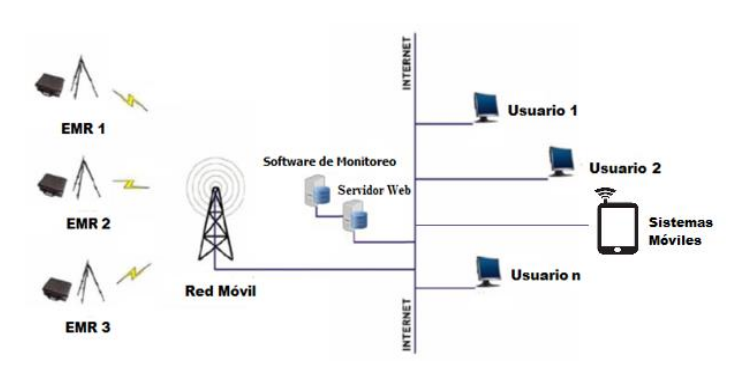
\includegraphics[width=0.6\textwidth]{../img/SMI_cartagena.png}
    \caption{Infraestructura típica de un sistema de monitoreo inteligente de ruido. Fuente: \cite{epacartagena2015}}
    \label{fig:diagrama-sistema-cartagena}
\end{figure}

}

\newenvironment{alcances}{
El presente proyecto se enfoca en el análisis del ruido generado en el área de los laboratorios del DEI, repasando los apartados vistos en la primera entrega que serán tomados en cuenta para esta segunda etapa del proyecto.

\begin{itemize}
    \item Medición de niveles de ruido: Se utilizarán sensores de sonido conectados a microcontroladores ESP8266 para captar datos acústicos en tiempo real en los diferentes laboratorios del DEI\ para monitorizar los ruidos generados por el alumnado.
    \item Generación de alertas: Cuando los niveles de ruido excedan el umbral permitido, el sistema enviará 
    notificaciones automáticas por correo electrónico. 
    \item Recolección y presentación de datos: Se implementara un servicio que almacenará y procesará los datos de sonido recogidos por los sensores, gestionará la información de reservas y administrará el envío de notificaciones. Asimismo, se desarrollará una interfaz web que permitirá visualizar los niveles de ruido por zona, gestionar configuraciones y consultar registros históricos.
    \item Cobertura de monitoreo: el dispositivo ESP8266 se implementará su instalación en el área de los laboratorios del DEI, el monitoreo empezará a recopilar cuando el laboratorio no se encuentra reservado para su uso. 
\end{itemize}

}{}
\newenvironment{limitaciones}{
El sistema busca ofrecer una solución efectiva para el monitoreo de ruido en los laboratorios, sin embargo, existen ciertas limitaciones que deben considerarse:

\begin{itemize}
    \item Precisión de los sensores: Al ser sensores de uso educativo, tienen limitantes por ejemplo en la
    calibración, la resolución y la sensibilidad a interferencias de otros ruidos ambientales. 
    \item Dependencia de la API de la universidad: La disponibilidad y estabilidad de la API interna de la
    universidad pueden afectar la obtención de datos en tiempo real sobre la existencia y el estado
    de reservas en las zonas configuradas.
    \item Tiempo de desarrollo: Debido a las limitaciones de tiempo para la ejecución del proyecto,
    se priorizaron las funcionalidades esenciales, dejando mejoras y optimizaciones para futuras
    iteraciones.
\end{itemize}

}{}
\newenvironment{objetivogeneral}{Desarrollar e implementar un sistema de monitoreo de ruido basado en tecnología IoT en la Universidad Centroamericana ``José Simeón Cañas`` (UCA), integrando el prototipo existente con los servicios institucionales, para garantizar la recolección, análisis y visualización de datos en tiempo real, permitiendo generar alertas oportunas al personal administrativo sobre niveles elevados de ruido en los espacios designado.
}{}
\newenvironment{objetivosespecificos}{
\begin{itemize}
    \item Vincular el dispositivo de monitoreo de ruido de la UCA a los servidores institucionales para el almacenamiento y gestión de datos en tiempo real.
    \item Diseñar y fabricar una cubierta para el dispositivo que asegure durabilidad, practicidad y buen funcionamiento del dispositivo.
    \item Completar la soldadura y el ensamblaje final del prototipo, asegurando que el dispositivo funcione correctamente.
    \item Implementar un módulo de análisis de datos que procese y visualice los niveles de ruido registrados, permitiendo la interpretación clara de la información y la toma de decisiones oportunas.
\end{itemize}

}{}

%=================================================================
%                Sección editable para capítulos
% ================================================================
% ================= NO MODIFICAR LOS COMANDOS ====================
% ================================================================

\newcommand{\capitulos}{
    
\capitulo{Marco teórico}{  
\section{¿Qué es el ruido?}

El término ``ruido`` significa simplemente ``ruidos molestos``. El ruido ambiental incluye, por ejemplo, el ruido del tráfico (vehículos de motor, trenes, aviones), el ruido industrial (máquinas) o el ruido del ocio (gritos fuertes o música, etc.). Sin embargo, la evaluación de la música en particular depende obviamente en gran medida de la percepción subjetiva; si es agradable, se llama "sonido" - de lo contrario "ruido". Dependiendo del país, hay diferentes regulaciones y leyes para regular el ruido ambiental. 

Éstos se diferencian entre distintos niveles, empezando por los ruidos molestos que perturban las actividades humanas o la vida silvestre, aumentan los niveles de estrés o de agresión o conducen a la alta presión sanguínea. En casos extremos, los niveles de ruido muy altos pueden tener efectos negativos duraderos en la salud, como la pérdida de audición, el tinnitus, los trastornos del sueño, el estrés agudo, los trastornos cardiovasculares o las enfermedades vasculares. En la naturaleza, el ruido provoca un aumento de la tasa de mortalidad tanto en los animales de presa como en los herbívoros debido a una percepción deteriorada, un comportamiento de apareamiento alterado o a la pérdida del sentido de orientación o de la audición.
            
\section{El impacto del ruido fuerte en la salud}
                    
 La contaminación sónica es uno de los grandes problemas en la sociedad moderna a escala mundial.
            
 El reconocimiento del ruido como un peligro para la salud es reciente y sus efectos han pasado a ser considerados un problema sanitario cada vez más importante. Dicha contaminación es la primera causa de contaminación ambiental en Francia, y la segunda en toda Europa. De forma global, Japón es el país más ruidoso del mundo, seguido de España,considerando a Madrid una de las capitales más ruidosas en todo el mundo, según estudios realizados por la OMS.
        
El ruido se define como un sonido indeseable, el sonido viaja en forma de ondas en el medio aéreo (o los cambios de presión) lo que produce la vibración del tímpano, el tímpano transfiere estas vibraciones a tres huesos minúsculos en el oído medio,los que a la vez comunican las vibraciones al fluido contenido en la cóclea (en el oído interno) Dentro de la cóclea se hallan las pequeñas terminales nerviosas usualmente conocidas como células ciliadas. Ellas responden a las vibraciones del fluido enviando los impulsos nerviosos al cerebro que entonce interpreta los impulsos como sonido o ruido.
           \begin{figure}[H]
            \centering
              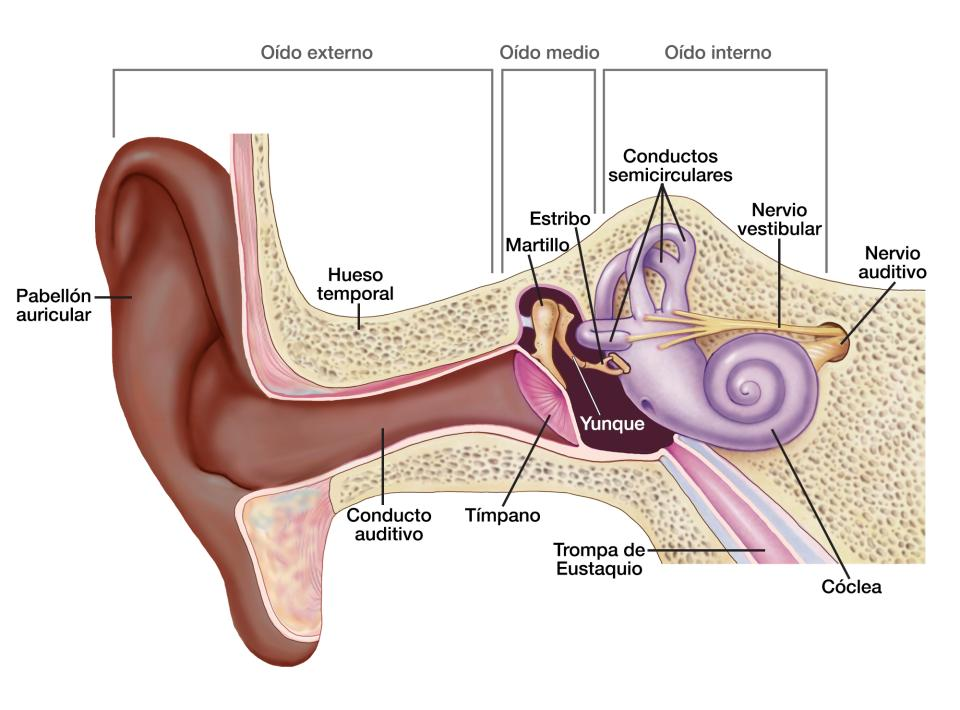
\includegraphics[width=0.7\textwidth]{../img/Oido.jpg}
              \caption{Partes del oído. Fuente: [NHJNIDCD 2022]}
              \label{fig:oido}
              \end{figure} 
        
 El ruido es considerado un peligro para la salud humana y sus efectos son catalogados como un problema sanitario cada vez más agravante. Puede causar desde insomnio, ansiedad, depresión, estrés, entre otros efectos psicológicos, hasta la pérdida parcial o total de la audición. Un ambiente que sobrepase los 55 decibelios (dB) es considerado un ambiente ruidoso, de 75 a 100dB es considerado un ambiente con ruido fuerte y superior a los 100dB es considerado un ambiente con ruido intolerable.
 
\subsection{Normativa de ruido según la OMS}

Más de 1000 millones de personas de edades comprendidas entre los 12 y los 35 años corren el riesgo de perder la audición debido a la exposición prolongada y excesiva a música fuerte y otros sonidos recreativos, lo que puede acarrear consecuencias devastadoras para su salud física y mental, educación y perspectivas de empleo.

En la Norma mundial para la escucha segura en lugares y eventos de entretenimiento se subrayan seis recomendaciones para velar por que dichos lugares y eventos limiten el riesgo de pérdida de audición entre sus clientes sin perder por ello la alta calidad del sonido y que la experiencia deje de ser agradable. Son las seis recomendaciones siguientes: 

 \begin{itemize}
     \item Un nivel sonoro medio máximo de 100 decibelios
     \item Seguimiento y registro constante de los niveles sonoros con equipos calibrados por personal designado a tal efecto
     \item Optimización de la acústica y los sistemas de sonido de la sala para garantizar una calidad de sonido agradable y una escucha segura
     \item Entrega al público de protección auditiva personal, junto con instrucciones de uso
     \item Acceso a zonas silenciosas para que los oídos descansen y disminuir el riesgo de daño auditivo.
     \item Formación de los trabajadores y distribución de información entre ellos.
 \end{itemize}

La nueva norma se ha elaborado en el marco de la iniciativa de la OMS Escuchar sin riesgos, que tiene por objeto mejorar las prácticas de escucha, especialmente entre los jóvenes, apoyándose en las últimas evidencias y en consultas con diferentes partes interesadas, como expertos de la OMS, los gobiernos, la industria, los consumidores y la sociedad civil \parencite{WHO2022}.  


\section{Contaminación sonora y sus consecuencias}

En la investigación previa (fase 1) de este trabajo de graduación se establecieron las bases teóricas sobre el problema que representa la contaminación acústica, cómo se identifica, cuál es el origen o los factores que originan mayormente la contaminación auditiva, estándares internacionales del límite permisible o tolerable para los seres humanos en el estándar de medición de rudio (decibelios) y las consecuencias que trae consigo la contaminación auditiva \parencite{carpio2025}. Si ahondamos un poco en el tema, son muchas las consecuencias tanto leves como graves las que se generan por permitir o mantener la contaminación auditiva en un entorno de aprendizaje como lo es el campus UCA.

Una investigación y trabajo técnico identificado como "Afectación del ruido ambiental a Instituciones Educativas; conjunto de acciones desde la Participación Ciudadana y Centros Educativos" en Ecuador evidencia que la contaminación acústica es o ruido ambiental como ellos suelen nombrarlo en su investigación desfavorece el rendimiento de estudiantes y además de docentes, causando fatigas, estŕes y problemas de concentración, destacando que la percepción de la afectación del ruido entre alumnos y maestros es:

Para maestros:
\begin{itemize}
\sloppy
    \item El ruido es contaminante que afecta al estado de ánimo e  interfiere con las actividades.
    \item El ruido provoca dolor de cabeza, estrés e irritabilidad.
    \item El ruido provoca afonías y dolores de garganta en el  profesorado al tener que elevar la voz.
    \item El trafico vehicular es un problema que genera contaminación del aire y ruido por sus motores y claxon.
    \item Informar, educar y concientizar son elementos claves para minimizar la problemática
    \item La sociedad en su conjunto es responsable de poner en práctica medidas para abatir la problemática.
\end{itemize}

Para alumnos:
\begin{itemize}
\sloppy
    \item El ruido es un problema que interfiere con las actividades
    \item El ruido provoca dolor de cabeza y distracción.
    \item El ruido provoca menor rendimiento escolar y, por lo  tanto, mayor fracaso.
    \item Ven incrementado drásticamente su nivel de irritabilidad  y agresividad.
    \item El ruido produce más dificultades para niños con necesidades educativas especiales.
    \item Atendiendo medidas disciplinares en casa y escuela, y con  no gritar contribuyo a disminuir la problemática.
\end{itemize}

Además destacan que la contaminación acústica incide de manera directa en la formación de los estudiantes, atentando de manera negativa en el rendimiento escolar, debido a que un sonido no deseado es capaz de captar la atención de las personas de forma involuntaria, se crea una distracción, perdiendo la concentración en la tarea que se realizaba. Resaltan que la contaminación acústica ha aumentado significativamente en los últimos y su incremento se debe a factores tales como: crecimiento poblacional, incremento de actividades utilizando métodos mecánicos, y el uso masivo de vehículos. 

La contaminación acústica incide de manera directa en la calidad y estilo de vida de la población, ejemplo de esto es la influencia de la contaminación acústica en las comunidades afectando aspectos cotidianos como la comunicación oral, el sueño, la concentración y el aprendizaje primordialmente. 

Inclusive dicha investigación contó que una recolección y muestreo de datos para poder validar la hipótesis implícitamente planteada sobre las consecuencias de la contaminación acústica y su afectación en el aprendizaje. El muestreo reveló que la mayor parte de los individuos inmiscuidos en el área académica (maestros y alumnos) reconocen que la contaminación acústica les ha afectado y seguirá afectado sus métodos de aprendizaje y desarrollo académico y que es necesario tomar medidas de prevención tales como realizar campañas informativas sobre la contaminación acústica, sus consecuencias y maneras de prevención, jornadas educativas para comprender los efectos negativos de la contaminación auditiva, desarrollar hábitos para respetar y perdurar el silencio en entornos de desarrollo académico y grupos de trabajo conformados por jóvenes y docentes capacitados en la prevención de la contaminación acústica para maximizar el alcance de la educación sobre prevención y reducción de la contaminación auditiva. \parencite{duque2023}

\section{Efecto del ruido en los estudiantes y su aprendizaje} 

Como situación internacional, una investigación realizada en 2002 por el doctor Alain Muzet, del Centro de Estudios Bioclimáticos en Francia, demostró que los niños cuyos centros escolares se encuentran próximos a zonas ruidosas (industrias, aeropuertos o carreteras con alto tránsito) presentan mayores dificultades en el aprendizaje de la lectura, muestran niveles más altos de  agresividad y fatiga, son más propensos a las peleas y riñas, tienden al aislamiento y experimentan problemas en sus relaciones sociales \parencite{marcelo2009ruido}.

El sonido ha sido definido como movimiento; sin movimiento no hay sonido. La vida cotidiana está rodeada de estímulos sonoros, lo que convierte al mundo en un entorno eminentemente acústico. Este entorno es relevante porque la información auditiva que perciben los individuos puede verse distorsionada si contiene errores, lo cual afecta directamente a la cognición y, en consecuencia, al aprendizaje. Por ello, el ruido puede vincularse con el rendimiento académico de los estudiantes. Entre los efectos identificados en niños en etapa preescolar y escolar se encuentran los siguientes:

\begin{itemize}
    \item \textbf{Deterioro auditivo}: la exposición continua a ruidos intensos afecta los umbrales de audición, obligando a los niños a escuchar físicamente menos sonidos. Este fenómeno es provocado principalmente por juguetes ruidosos y equipos presentes en su entorno. Se ha determinado que el deterioro auditivo comienza a manifestarse a partir de los 70 dB(A).
    \item \textbf{Alteraciones del sueño}: en condiciones experimentales se ha observado que los niños expuestos a ruidos de hasta 95 dB durante la fase REM presentan variaciones significativas en su patrón de descanso, lo cual afecta su recuperación física y mental.
    \item \textbf{Efectos somáticos relacionados con el estrés:} la exposición al ruido del tráfico, tanto dentro como fuera de las aulas, incrementa la presión sanguínea sistólica y diastólica, lo que genera consecuencias fisiológicas asociadas al estrés.
    \item \textbf{Efectos cognitivos en la lectura:} diversos estudios han demostrado una correlación negativa entre la exposición al ruido y el desarrollo de habilidades lectoras en los niños, dificultando así la adquisición de competencias fundamentales para el aprendizaje.
    \item \textbf{Memoria:} investigaciones han mostrado que la exposición al ruido de aviones, incluso en simulaciones de corta duración (15 minutos, con intensidades de 55 a 66 dB), afecta la retención de la memoria a corto y largo plazo, particularmente en tareas de tipo visual.
    \item \textbf{Atención}: los niños sometidos a altos niveles de ruido experimentan dificultades en la codificación visual de objetos y en el tiempo que logran mantener la concentración en actividades específicas, como la discriminación auditiva o visual.
    \item \textbf{Motivación:} tanto estudios de laboratorio como de campo han revelado que la exposición crónica al ruido reduce la motivación en los niños, quienes se muestran menos dispuestos a enfrentar situaciones desafiantes o prolongadas. Además, se ha observado que el ruido incrementa los niveles de frustración durante la ejecución de tareas.
\end{itemize}

Finalmente, diversos autores señalan que los mecanismos y procesos subyacentes afectados por el ruido incluyen la percepción, el habla y la adquisición del lenguaje, lo cual repercute negativamente en el aprendizaje de la lectura y en procesos cognitivos de mayor complejidad, como la memoria a largo plazo y la comprensión semántica.

En el caso de niños sin alteraciones auditivas congénitas, se ha encontrado una fuerte correlación entre el ruido del tráfico y la capacidad de discriminar el habla. Asimismo, la exposición prolongada a entornos ruidosos influye en el desarrollo de estrategias cognitivas para “ignorar” el ruido ambiental; sin embargo, este mecanismo no solo reduce la percepción de sonidos molestos, sino que también limita la capacidad de captar información relevante para el aprendizaje.

\section{Sistema de monitoreo de ruido}
En la fase 1 de este proyecto, se menciona acerca de la salud auditiva, el concepto del ruido y la medición del ruido utilizando la escala estandarizada basada en la unidad logarítmica para medir el sonido que son los decibelios (dB) \parencite{carpio2025}. Un sistema de monitoreo de ruido como tal concatena diversos términos y conocimientos a tomar en cuenta como lo son los siguientes: 

\begin{itemize}\setlength{\itemsep}{0.8em}

    \item \textbf{Monitoreo del ruido.} El monitoreo del ruido implica el control del sonido a largo plazo sin necesidad de interacción humana. Hay dos tipos principales de control del sonido: el control del lugar de trabajo y el control del ruido ambiental, cada uno de los cuales depende de la ubicación de la fuente de sonido. El monitoreo del ruido ambiental es uno de los tipos más comunes de vigilancia del medio ambiente y se lleva a cabo con mayor frecuencia mediante un sistema de monitoreo \parencite{Svantek2025MonitoreoDelRuido}.

    \item \textbf{Sistema de monitoreo de ruido.} El sistema de monitoreo, tal como se describe en la norma ISO 1996-2, comprende un monitor de ruido y un centro de recogida de datos, así como todo el hardware y el software utilizados para el monitoreo del ruido ambiental \parencite{Svantek2025MonitoreoDelRuido}. Un sistema de monitoreo de ruido en línea es una tecnología avanzada que permite detectar y analizar continuamente los niveles de ruido en diversos contextos. Mantener este sistema en funcionamiento es fundamental para cumplir con las restricciones de ruido, especialmente en entornos urbanos, industriales y de construcción. Las ventajas de este enfoque son que no es necesario instalar ningún software, se puede acceder a los informes desde cualquier lugar con conexión a Internet y se pueden compartir los resultados fácilmente \parencite{AdvanceTech2024}.

    \item \textbf{Monitor de ruido.} El término monitor de ruido, también llamado ``Terminal de Monitoreo de Ruido`` (NMT), se refiere a la instrumentación utilizada para el monitoreo continuo automatizado del sonido, que registra los niveles de presión sonora ponderados A, sus espectros y todas las cantidades meteorológicas relevantes como velocidad y dirección del viento, lluvia, humedad y estabilidad atmosférica \parencite{Svantek2025MonitoreoDelRuido}. El objetivo de un monitor de ruido es proporcionar datos sobre el nivel de ruido en un lugar para poder compararlo con los límites establecidos. En nuestro caso, el sensor MAX9814 funge como monitor de ruido, cuyas características y capacidades se mencionaron en la fase 1 de este trabajo \parencite{carpio2025}.
 \begin{figure}[H]
   \centering
   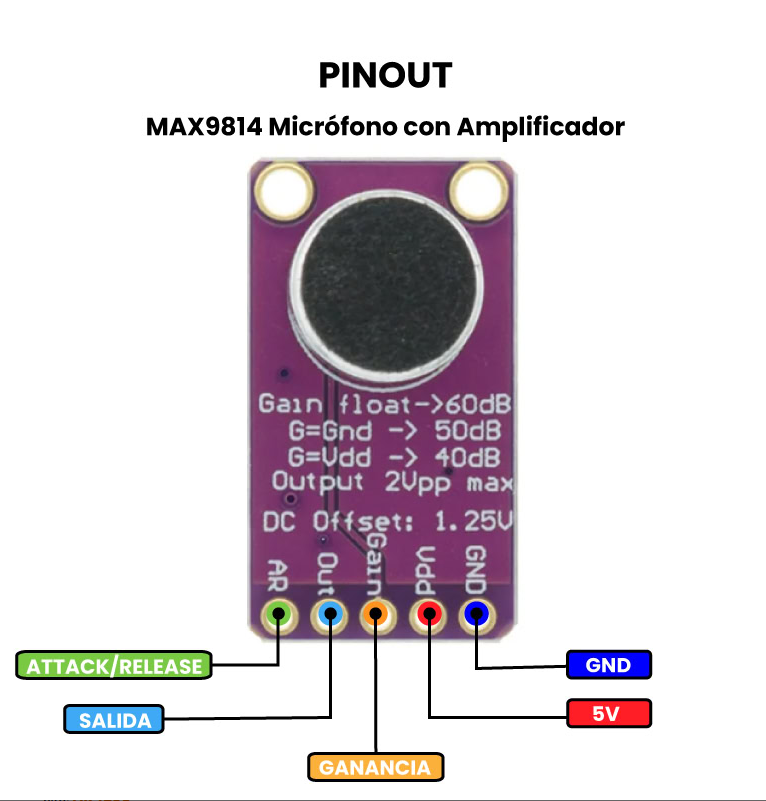
\includegraphics[width=0.7\textwidth]{../img/sensor_MAX.png}
   \caption{Sensor MAX9814 Amplificador de micrófono. Fuente: \url{https://uelectronics.com/producto/max9814-microfono-con-amplificador}}
   \label{fig:sensorMAX}
 \end{figure}

    \item \textbf{Vigilancia del ruido.} El monitoreo del ruido debe ocurrir siempre que exista el riesgo de sobrepasar los límites de los niveles de ruido. Como resultado de los estudios sobre las conexiones entre el ruido y la salud, así como de los procedimientos de elaboración de políticas en varios países, los gobiernos han establecido valores límite nacionales y reglamentos para el ruido ambiental. Dependiendo de la normativa local, los límites de dB permitidos para el ruido ambiental pueden variar. Normalmente, para el día, el límite de dB permitido es de 65 dBA, y para los niveles de ruido nocturnos, de 55 dBA. El control de la calidad del ruido es el proceso de vigilancia continua de los niveles de ruido en un entorno para garantizar que se mantienen dentro de los límites aceptables \parencite{Svantek2025MonitoreoDelRuido}.
\end{itemize}

\section{Beneficios de un sistema de monitoreo de ruido}

Dado que la monitorización de ruido representa en general una medida de prevención y reducción de la contaminación sonora, existen más beneficios en cuanto al rendimiento, fiabilidad y facilidad de uso de estos sistemas (para el caso de nuestro trabajo aplican los beneficios a mencionar), estos son: 

\begin{itemize}

    \item \textbf{Alertas y notificaciones:} El sistema puede configurarse para enviar correos electrónicos o alertas SMS a los administradores del sistema de monitoreo cuando los niveles de ruido superan los límites establecidos, lo que garantiza que los niveles de ruido excesivos se reduzcan rápidamente \parencite{AdvanceTech2024}
    \vspace{1cm}
    \item \textbf{Acceso y control remotos:} Con conectividad a Internet, estos sistemas permiten el acceso remoto a los datos de ruido, lo que permite a los usuarios monitorear y administrar los niveles de ruido desde cualquier ubicación. \parencite{AdvanceTech2024}
    \vspace{1cm}
    \item \textbf{Monitoreo en tiempo real:} El sistema registra continuamente los niveles de ruido, proporcionando actualizaciones en tiempo real que ayudan en la evaluación y respuesta inmediata a la contaminación acústica. \parencite{AdvanceTech2024}
    \vspace{1cm}
    \item \textbf{Registro y análisis de datos:} Registra automáticamente los datos de ruido a lo largo del tiempo, lo que facilita el análisis detallado y la generación de tendencias de los niveles de ruido. Esta función es esencial para comprender patrones e identificar fuentes específicas de ruido. \parencite{AdvanceTech2024}. Para el caso de este proyecto en la fase 1 se demostró que con los datos recopilados a lo largo del tiempo se generan y muestran gráficos de barras y líneas con los datos recopilados facilitan la comprensión de las tendencias de aumento y decremento de sonidos en los laboratorios del departamento de electrónica e informática \parencite{carpio2025}
    
            \begin{figure}[H]
             \centering
              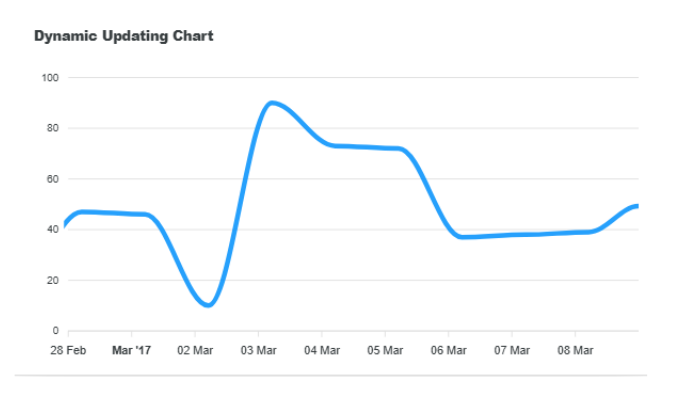
\includegraphics[width=0.7\textwidth]{../img/grafico_linea.png}
              \caption{Componente de gráfica de línea. Fuente: \parencite{carpio2025}}
              \label{fig:your_label}
            \end{figure} 

            \begin{figure}[H]
              \centering
              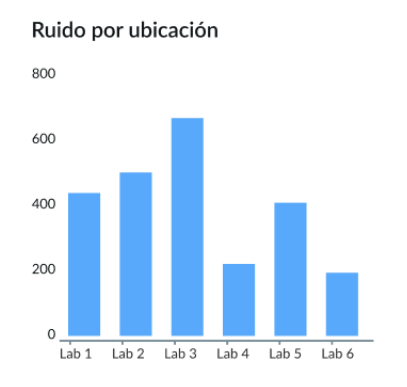
\includegraphics[width=0.7\textwidth]{../img/grafico_barras.png}
              \caption{Componente de gráfica de barras. Fuente: \cite{carpio2025}}
              \label{fig:your_label}
            \end{figure}
    
\end{itemize}

\section{Websockets}

\subsection{¿qué es un websocket?}

WebSockets es una tecnología basada en el protocolo ws, este hace posible establecer una conexión continua full-duplex, entre un cliente y servidor. Un cliente websocket podría ser el navegador del usuario, pero el protocolo es una plataforma independiente. Un servidor WebSocket es simplemente una aplicación TCP que escucha en cualquier puerto de un servidor que sigue un protocolo específico. Un servidor WebSocket puede ser escrito en cualquier lenguaje de programación Server-Side que sea soporte Berkeley Sockets, como por ejemplo C++ o Python o inclusive PHP y JavaScript para servidores.   

}
    \capitulo{Metodología}{
    
  \section{ Metodologia Scrum }

Scrum es un proceso en el que se aplican de manera regular un conjunto de buenas prácticas para trabajar colaborativamente, en equipo, y obtener el mejor resultado posible de un proyecto. Estas prácticas se apoyan unas a otras y su selección tiene origen en un estudio de la manera de trabajar de equipos altamente productivos  \parencite{scrum2021} . 

En Scrum se realizan entregas parciales y regulares del producto final, priorizadas por el beneficio que aportan al receptor del proyecto. Por ello, Scrum está especialmente indicado para proyectos en entornos complejos, donde se necesita obtener resultados pronto, donde los requisitos son cambiantes o poco definidos, donde la innovación, la competitividad, la flexibilidad y la productividad son fundamentales. 

Scrum también se utiliza para resolver situaciones en que no se está entregando al cliente lo que necesita, cuando las entregas se alargan demasiado, los costes se disparan o la calidad no es aceptable, cuando se necesita capacidad de reacción ante la competencia, cuando la moral de los equipos es baja y la rotación alta, cuando es necesario identificar y solucionar ineficiencias sistemáticamente o cuando se quiere trabajar utilizando un proceso especializado en el desarrollo de producto. 

\subsection{Proceso SCRUM} 

En Scrum un proyecto se ejecuta en ciclos temporales cortos y de duración fija (iteraciones que normalmente son de 2 semanas, aunque en algunos equipos son de 3 y hasta 4 semanas, límite máximo de feedback de producto real y reflexión). Cada iteración tiene que proporcionar un resultado completo, un incremento de producto final que sea susceptible de ser entregado con el mínimo esfuerzo al cliente cuando lo solicite. 

 \begin{figure}[H]
  \centering
  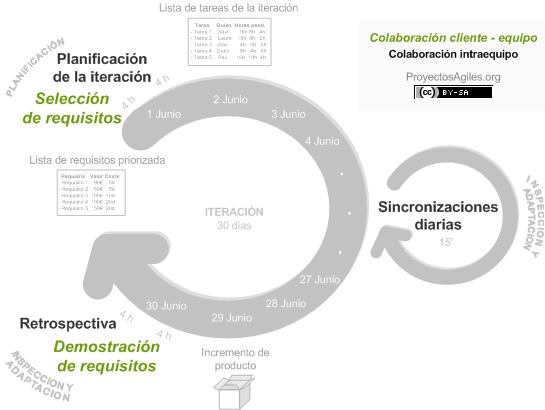
\includegraphics[width=0.7\textwidth]{../img/Metodologia Scrum.jpeg}
  \caption{Proceso Scrum. Fuente: [\cite{scrum2021}]}
  \label{fig:scrum}
  \end{figure} 

Cada día el equipo realiza una reunión de sincronización (15 minutos), normalmente delante de un tablero físico o pizarra (Scrum Taskboard). El equipo inspecciona el trabajo que el resto está realizando (dependencias entre tareas, progreso hacia el objetivo de la iteración, obstáculos que pueden impedir este objetivo) para poder hacer las adaptaciones necesarias que permitan cumplir con la previsión de objetivos a mostrar al final de la iteración. En la reunión cada miembro del equipo responde a tres preguntas: 

\begin{itemize}
    \item ¿Qué he hecho desde la última reunión de sincronización para ayudar al equipo a cumplir su objetivo?
    \item ¿Qué voy a hacer a partir de este momento para ayudar al equipo a cumplir su objetivo?
    \item ¿Qué impedimentos tengo o voy a tener que nos impidan conseguir nuestro objetivo?
\end{itemize}

Durante la iteración el Facilitador (Scrum Master) se encarga de que el equipo pueda mantener el foco para cumplir con sus objetivos. 
Elimina los obstáculos que el equipo no puede resolver por sí mismo. 
Protege al equipo de interrupciones externas que puedan afectar el objetivo de la iteración o su productividad. 

Durante la iteración, el cliente junto con el equipo refinan la lista de requisitos (para prepararlos para las siguientes iteraciones) y, si es necesario, cambian o replanifican los objetivos del proyecto (10\% -- 15\% del tiempo de la iteración)
 con el objetivo de maximizar la utilidad de lo que se desarrolla y el retorno de inversión. 

Todo esto ayudo a que pudieramos tener una mejor organización en las tareas a realizar, la cooperación de cada integrante del equipo y supervisar que las tareas se realizarán en el tiempo establecido, garantizando así un trabajo exitoso.
 \subsection{Organización}
 La estructura organizacional que el equipo adopto para este proyecto se definió bajo el enfoque de la metodología Scrum, estableciendo funciones claras y tareas específicas dependiendo de las habilidades de cada integrante del proyecto. Los roles que se definieron dentro de la organizacion fueron ´
los siguientes:

\textbf{Roles Metodología Scrum }

\begin{itemize}
    \item Dueño del producto: Miguel Ernesto Rivas Serrano.
    \item Stakeholders: Miguel Ernesto Rivas Serrano.
    \item Facilitador del proceso Scrum (Product Owner): José Heriberto Olivares Barrientos.

\item {Equipo de desarrollo: }

\end{itemize}
\vspace{1em}

\begin{table}[H]
\centering
\caption{Roles SCRUM}
\label{tab:roles}

\renewcommand{\arraystretch}{1.3} 
\begin{tabular}{|p{5cm}|p{8cm}|} 
\hline
\textbf{Responsable} & \textbf{Rol} \\
\hline
José Heriberto Olivares Barrientos & Encargado de QA/Testing manual \\
\hline
Paula Daniela Zepeda Barrera & Encargada de QA/Testing manual \\
\hline
Julio Josué Chávez Flores & Encargado de QA/Testing automatizado, Modelador 3D y Técnico eléctrico \\
\hline
Marcos Antonio Hernández Grande & Encargado de QA/Testing automatizado \\
\hline
\end{tabular}

\vspace{0.5cm}
\centering
\small Fuente: [Elaboración propia]
\end{table}

En nuestro proceso Scrum acordamos realizar reuniones semanales entre una y dos veces por semana, con el objetivo de definir las tareas y metas a cumplir, así como elaborar un cronograma de actividades que facilite la organización y el desarrollo del proyecto.

El trabajo se estructuró en sprints con una duración de 1 a 2 semanas, según el nivel de complejidad de las actividades, y con una distribución colaborativa de tareas entre los integrantes del equipo.

Durante las reuniones, cada miembro compartía los avances logrados, las dificultades encontradas y se realizaba una revisión general del progreso del proyecto para asi lograr un resultado exitoso.

\section{Cronograma de Actividades}

 \vspace{1em}
  
   \begin{figure}[H]
        \centering
        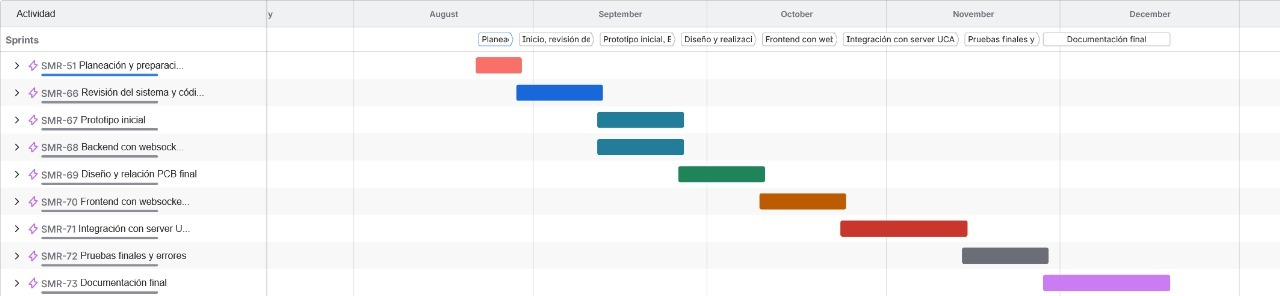
\includegraphics[width=0.7\textwidth]{../img/Cronograma .jpeg}
     \caption{Cronograma de actividades. Fuente: [Elaboración Propia]}
     \label{fig:cronograma1}
    \end{figure} 

    \begin{figure}[H]
    \centering
      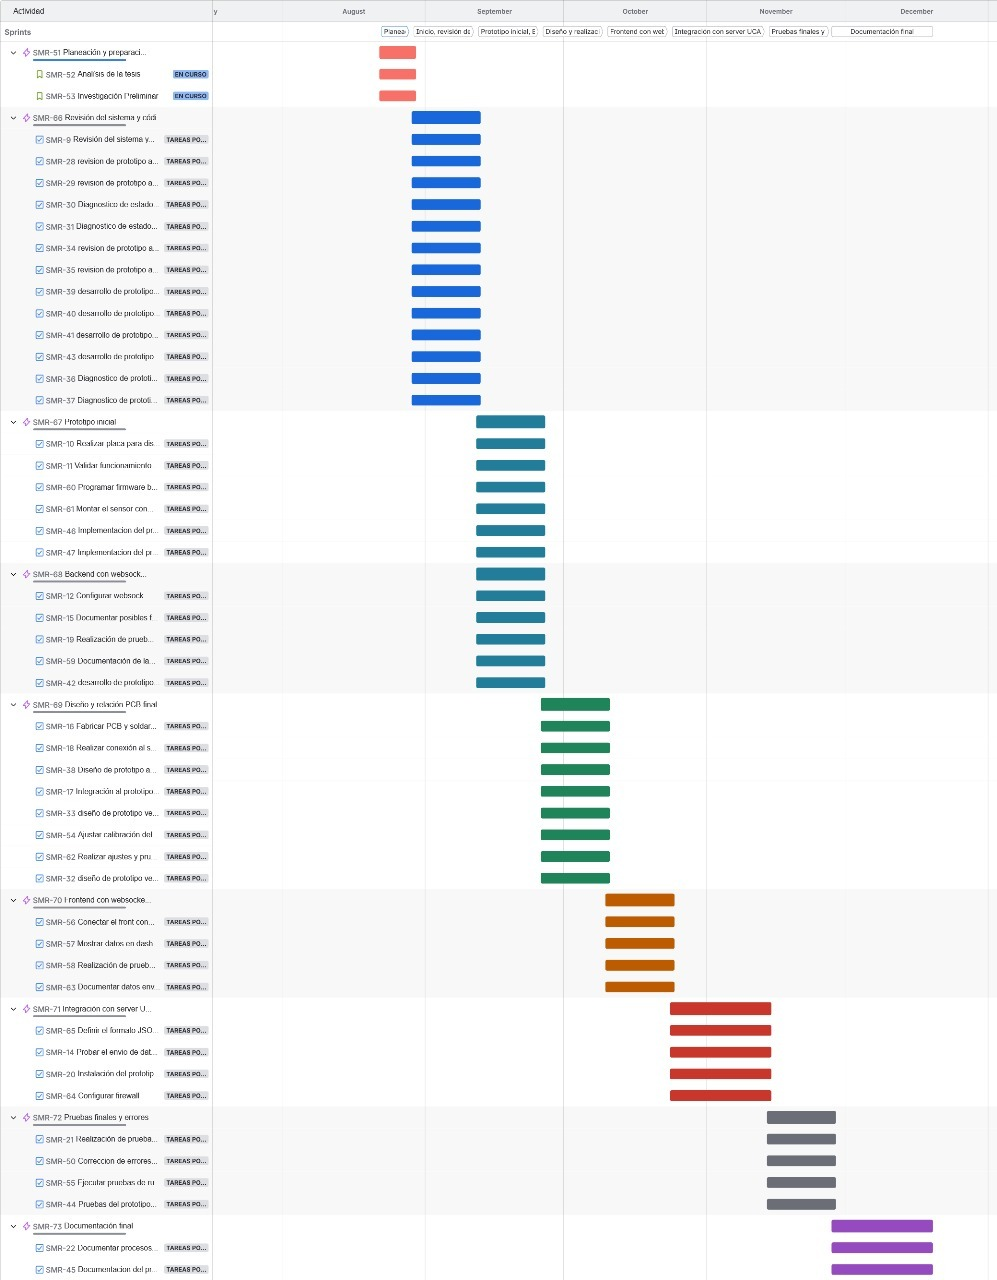
\includegraphics[width=0.7\textwidth]{../img/Cronograma 2.jpeg}
      \caption{Cronograma de actividades. Fuente: [Elaboración Propia]}
      \label{fig:cronograma}
       \end{figure}


}
\capitulo{Presentación, análisis e interpretación de resultados}{
    En esta sección de debe explicar cómo los resultados se derivan de las mediciones realizadas. Pueden añadirse diagramas para clarificar el diseño experimental, gráficos y tablas para ilustrar mejor los resultados. Por otra parte, en el análisis e interpretación de los resultados se debe responder a la pregunta planteada en la introducción. Es necesario hacer énfasis en porqué sus resultados son relevantes. Finalmente plantee las fortalezas y las debilidades de su estudio.
    }

    \capitulo{Formato de los trabajos}{
    A continuación, se muestran las características principales del formato de trabajos de graduación creado por la facultad de ingeniería y arquitectura de la UCA.
    
    \begin{lista}
        \item \textbf{Partes del documento:}
        \begin{lista}
            \item Primera portada.
            \item Segunda portada.
            \item Agradecimientos (opcional).
            \item Dedicatorias (opcional).
            \item Resumen.
            \item Índice.
            \item Índice de figuras.
            \item Índice de tablas.
            \item Siglas.
            \item Abreviaturas.
            \item Nomenclatura.
            \item Capítulos.
            \item Glosario (opcional).
            \item Referencias.
            \item Anexos.
        \end{lista}

        \item \textbf{Formato general:}
        \begin{lista}
            \item Pagina tamaño carta.
            \item Margen de 2.5cm en todos lados.
            \item Borde de encuadernación de 1cm.
            \item Fuente Times New Roman 11pt.
            \item Interlineado 1.5pt.
            \item Espacio extra entre párrafos 0.
            \item Línea vacía entre párrafos.
            \item Todas las secciones deben comenzar en página impar.
            \item En todas las secciones que llevan título, el titulo se coloca al inicio de la página, en negrita, en mayúscula y centrado horizontalmente.
            \item Debe haber separación de una línea vacía entre el título y el texto.
        \end{lista}

        \item \textbf{Portadas:}
        \begin{lista}
            \item Texto centrado horizontalmente.
            \item Espacio igual entre los párrafos para que el texto ocupe todo el espacio disponible.
            \item Texto en mayúscula.
            \item Fuente tamaño 14pt.
            \item Logo de la primera portada 2.5cm de alto.
            \item En la primera portada los nombres de los integrantes van ordenados en orden alfabético basados en el primer apellido.
    \end{lista}

    \item \textbf{Agradecimientos:}
    \begin{lista}
        \item Extensión máxima una página.
    \end{lista}

    \item \textbf{Dedicatoria:}
    \begin{lista}
        \item Una por cada integrante.
        \item Extensión máxima una página.
        \item Debe llevar el nombre correspondiente del integrante al final de la página y alineado al lado derecho.
    \end{lista}

    \item \textbf{Resumen:}
    \begin{lista}
        \item Extensión de una a tres páginas.
    \end{lista}

    \item \textbf{Índice:}
    \begin{lista}
        \item El espacio horizontal entre el nombre de las secciones y el número de página debe estar lleno de puntos.
        \item Se permite hasta tres niveles de título.
        \item Los títulos de las secciones principales van en mayúscula.
        \item Al final se deben colocarlos anexos.
    \end{lista}

    \item \textbf{Índice de figuras e índice de tablas:}
    \begin{lista}
        \item Cada entrada del índice de figuras debe iniciar con la palabra “Figura” seguido del número de capitulo y el número correlativo de la figura.
        \item Cada entrada del índice de tablas debe iniciar con la palabra “Tabla” seguido del número de capitulo y el número correlativo de la tabla.
    \end{lista}

    \item\textbf{Siglas, abreviaturas y nomenclatura:}
    \begin{lista}
        \item Van separados en dos columnas, en la columna izquierda se coloca la sigla o palabra seguido de dos puntos y en la columna derecha se coloca la definición.
    \end{lista}

    \item\textbf{Figuras:}
    \begin{lista}
        \item Las figuras incluyen gráficos, diagramas, fotos, etc.
        \item El epígrafe va en la parte inferior centrado horizontalmente.
        \item Al inicio va la palabra “Figura” seguido del número de capitulo y número correlativo.
        \item En el epígrafe continuo a la descripción de la figura va la fuente.
        \item La fuente sigue el siguiente formato, “Fuente: [apellido autor, año]”.
        \item Si la figura es de elaboración propia se coloca, “Fuente: [Elaboración propia]”.
        \item Si la figura ha sido adaptada de alguna parte se coloca, “Adaptado de: [apellido autor, año]”.
        \item Las figuras se pueden colocar con orientación horizontal, en ese caso siempre de izquierda a derecha.
        \item Si la figura tiene orientación horizontal, el epígrafe se coloca en el lado derecho de la página.
    \end{lista}

    \item\textbf{Tabla:}
    \begin{lista}
        \item El epígrafe va en la parte superior, centrado horizontalmente.
        \item Al inicio va la palabra “Tabla” seguido del número de capitulo y número correlativo.
        \item La fuente se coloca en la parte inferior, centrada horizontalmente.
        \item La fuente sigue el siguiente formato, “Fuente: [apellido autor, año]”.
        \item Si la tabla es de elaboración propia se coloca, “Fuente: [Elaboración propia]”.
        \item Si la figura ha sido adaptada de alguna parte se coloca, “Adaptado de: [apellido autor, año]”.
        \item Las tablas se pueden colocar con orientación horizontal, en ese caso siempre de izquierda a derecha.
        \item Si la tabla tiene orientación horizontal, el epígrafe se coloca en el lado izquierdo de la página.
    \end{lista}

    \item\textbf{Ecuaciones:}
    \begin{lista}
        \item Las ecuaciones deben estar numeradas de la siguiente forma “(Ec.1.1)”.
    \end{lista}

    \item \textbf{Glosario:}
    \begin{lista}
        \item Tiene el mismo formato que las siglas, abreviaturas y nomenclatura.
    \end{lista}

    \item\textbf{Referencia:}
    
    \begin{lista}
        \item El formato de la referencia es en formato APA.
        \item No se coloca sangría en las líneas de cada una de las referencias.
        \item Las referencias van separadas horizontalmente por una línea vacía.
    \end{lista}

  

    \item\textbf{Portada anexos:}
    \begin{lista}
        \item Los anexos se enumeran utilizando letras.
        \item La portada de los anexos lleva dos partes, lleva la palabra “ANEXO” en mayúscula seguido de la letra correspondiente, el tamaño de fuente de esta parte es 20pt.
        \item El título del anexo en mayúscula, el tamaño de fuente de esta parte es 16pt.
        \item Todo el texto va centrado vertical y horizontalmente.
    \end{lista}

    \end{lista}
    }
}


%=================================================================
%       Sección editable para conclusiones y recomendaciones
% ================================================================
% ================= NO MODIFICAR LOS COMANDOS ===================
% ================================================================

\newenvironment{conclusiones}{En esta sección se escriben las conclusiones a las que se ha llegado luego de realizar el trabajo, las conclusiones deben concordar con los objetivos planteados anteriormente.}{}

\newenvironment{recomendaciones}{
En esta sección, se presentan las recomendaciones hechas por el grupo de trabajo para las personas que se beneficiarán del estudio o proyecto realizado.
}{}

%=================================================================
%                Sección editable para glosario
% ================================================================
% ================= NO MODIFICAR LOS COMANDOS ====================
% ================================================================

\newcommand{\mostrarglosario}{true}
\itemglosario{Glosario}{En esta sección, se incluyen términos utilizados en el documento cuya definición podría\newline no ser conocida por el lector, especialmente aquellos de carácter técnico. Esta sección\newline es opcional, como por ejemplo: BackEnd (Parte de una aplicación web que gestiona\newline la lógica, el procesamiento de datos y la comunicación con el servidor).}
\itemglosario{}{}
\itemglosario{}{}



%=================================================================
%                    Sección editable para anexos
% ===============================================================
% ================== NO MODIFICAR LOS COMANDOS ==================
% ================================================================

\newcommand{\anexos}{
    \anexo{anexos}{
     En los anexos se colocan los documentos, gráficos, tablas, imágenes u otros materiales complementarios que proporcionan información adicional relevante, pero que no forman parte del cuerpo principal del trabajo.
    }
}

